\subsubsection{Træning}
Efter brugeren har angivet sin helbredstilstand starter træningen. Før selve træningen kan påbegyndes, spørger systemet brugeren om, hvorvidt kompatible enheder skal tilkobles. Disse enheder kan eksempelvis være pulsmålere. Vælger brugeren ikke at tilkoble eksterne enheder, startes tiden og gps'en, og selve træningen kan påbegyndes. Vælger brugeren at tilkoble enheder, prøver systemet at synkronisere med enhederne, og hvis dette lykkes, påbegyndes selve træningen og alle måleenhederne starter.

Under træningen har brugeren mulighed for at


\\begin{figure} [H]
\centering
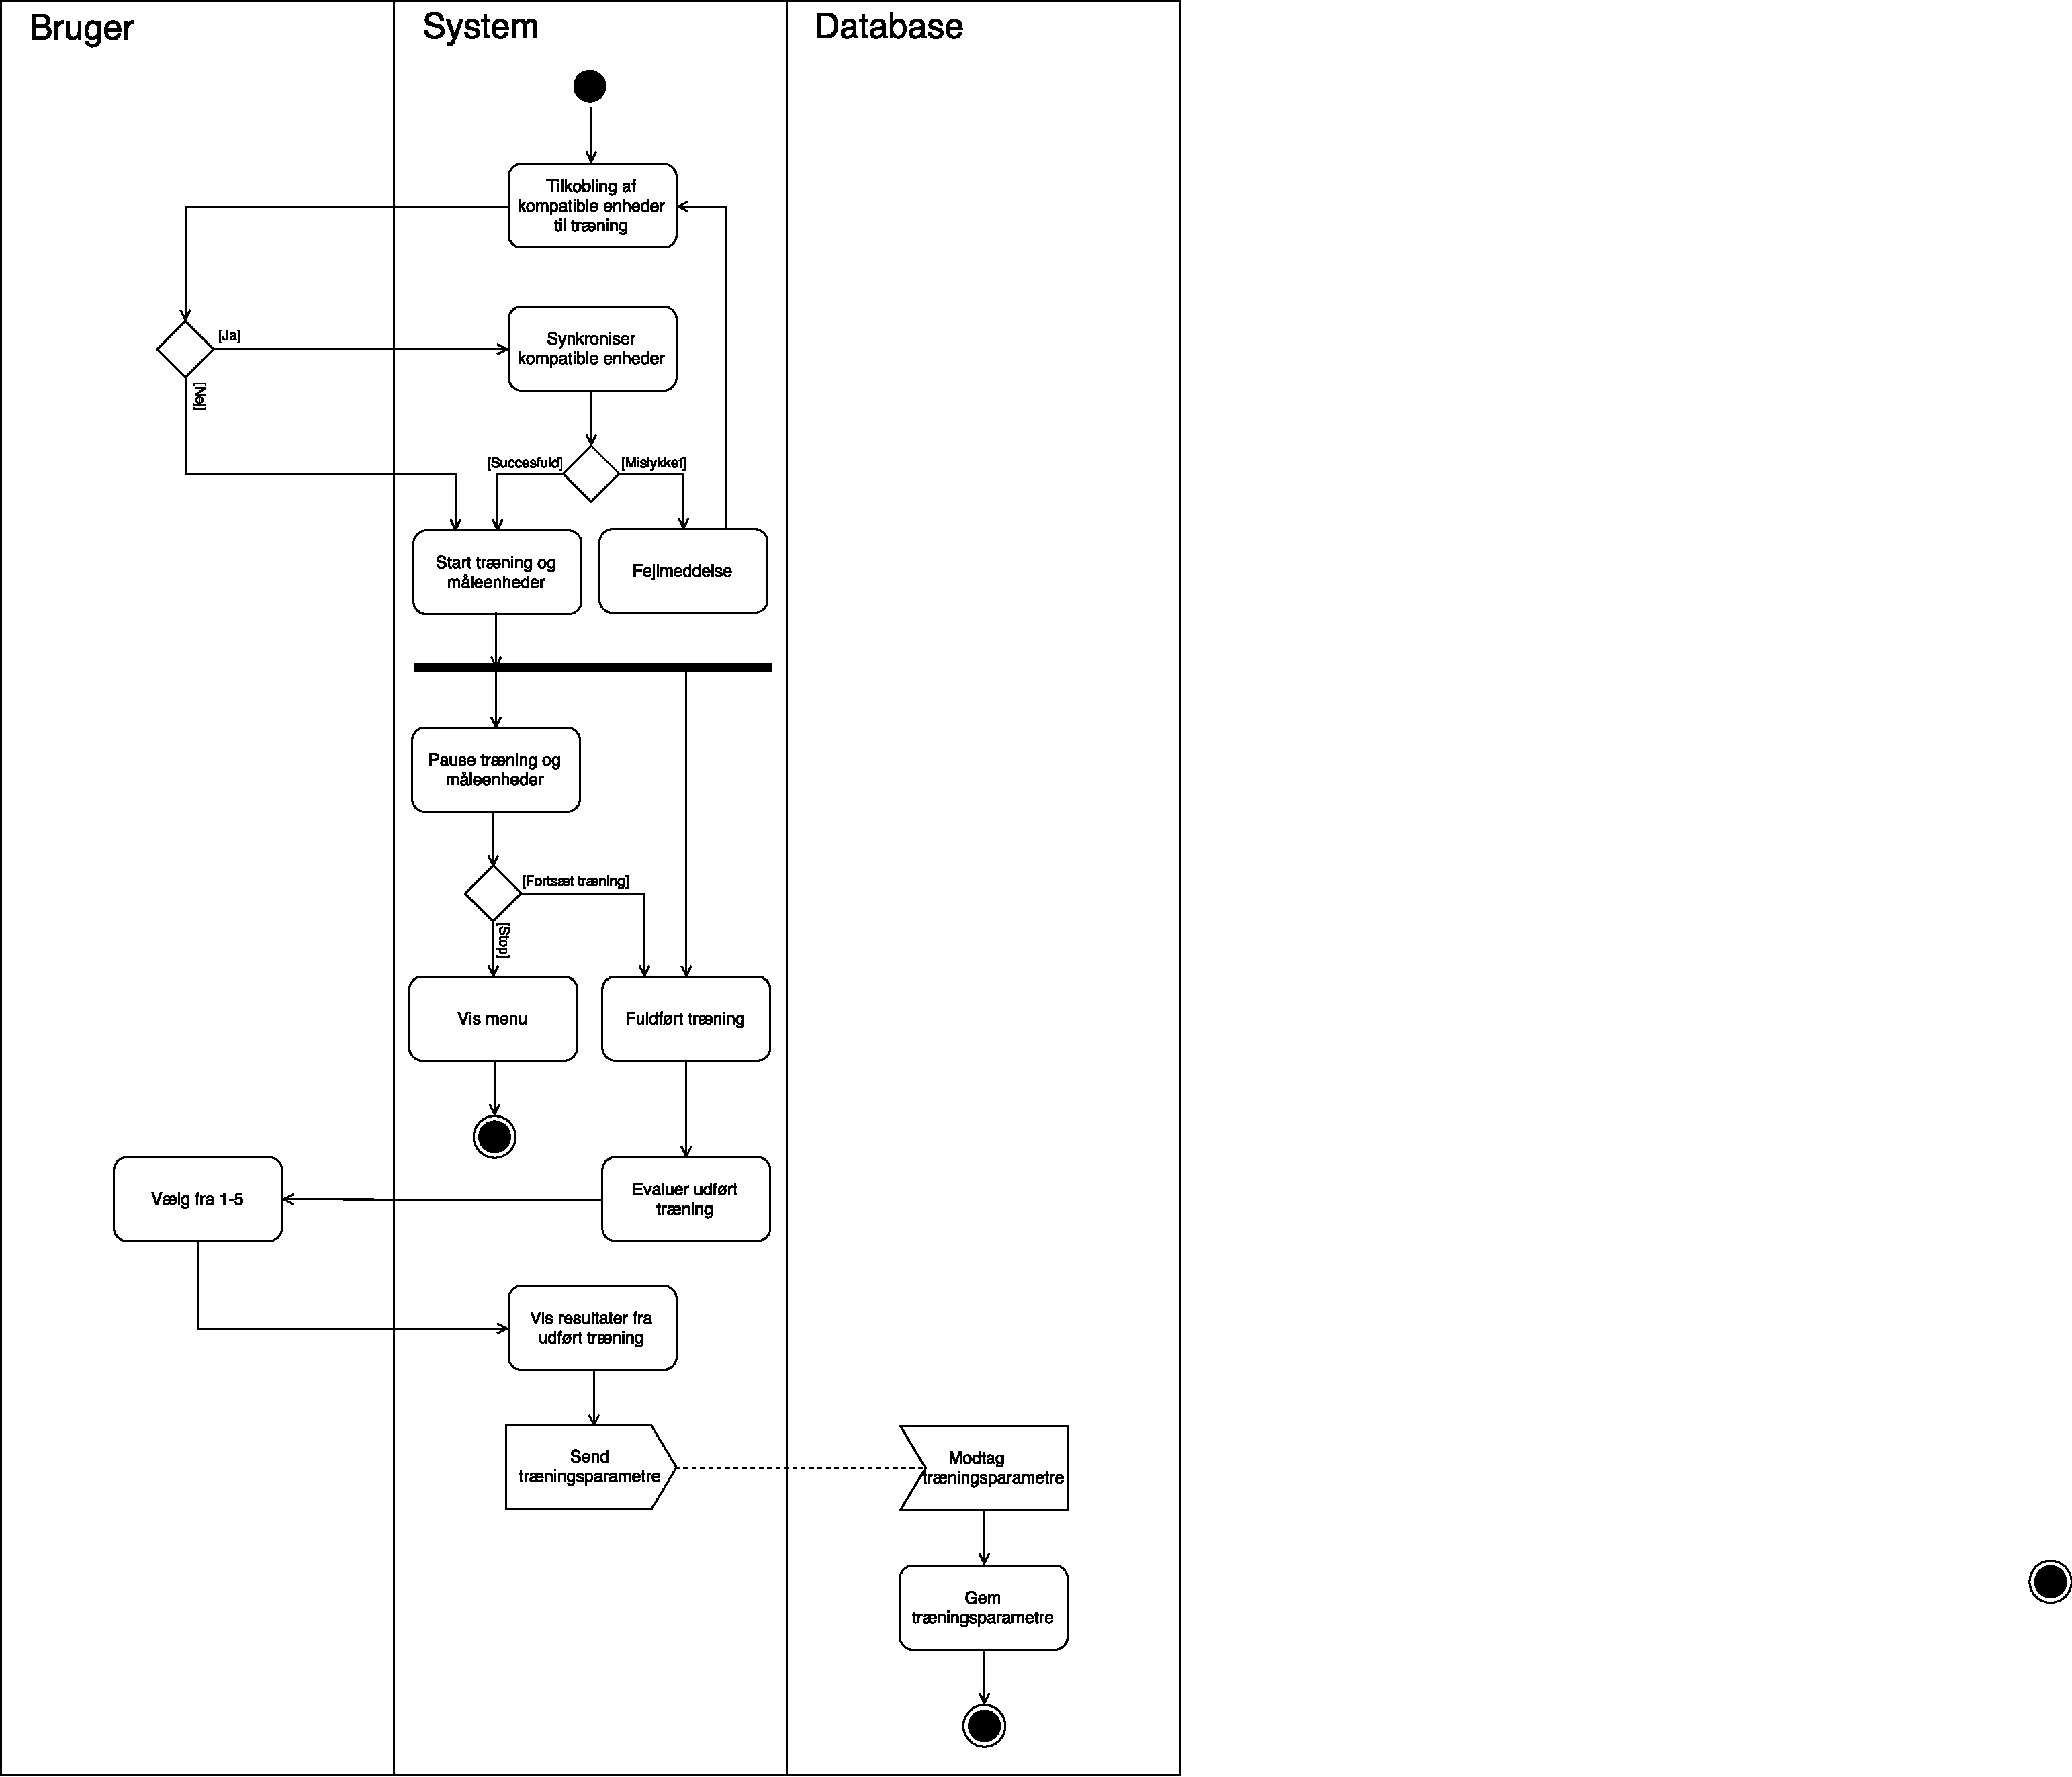
\includegraphics[width=0.9\textwidth]{figures/aktivitetsdiagram/Traening}
\caption{Aktivitetsdiagram over træning.}
\label{fig:resultater}
\end{figure}

\noindent